\documentclass[12pt]{mpllatex}
\usepackage{examples}
\usepackage{caption}
\usepackage{pgfplots}

\begin{document}

\section*{Plotting Bessel functions}

This simple example uses Maple to produce a plot of the first six Bessel functions. Two plots are shown, one created by Maple and a second created by LaTeX using the plotting package {\tt\small pgfplots} and the data exported from Maple.

\begin{maple}
   with(plottools):

   myPlot := plot([seq(BesselJ(i, z), i = 0 .. 5)], z = 0 .. 15):

   exportplot("example-04-fig.jpeg",myPlot,"JPEG"):   # Maple18

   a,b,n := 0.0,15.0,150:           # domain and number of samples
   dx := (b-a)/n:                   # uniform step

   fd := fopen ("example-04.txt", WRITE):
   for i from 0 to n by 1 do
      x := a + dx*i:
      fprintf(fd,"% .10e % .10e % .10e % .10e % .10e % .10e % .10e\n",x,
                 seq(evalf(BesselJ(k,x)),k=0..5)):
   end do:
   fclose(fd):
\end{maple}

\clearpage

\hrule height0pt
\vfill
\begin{minipage}{\textwidth}
   \centering
   \IfFileExists{example-04-fig.jpeg}%
   {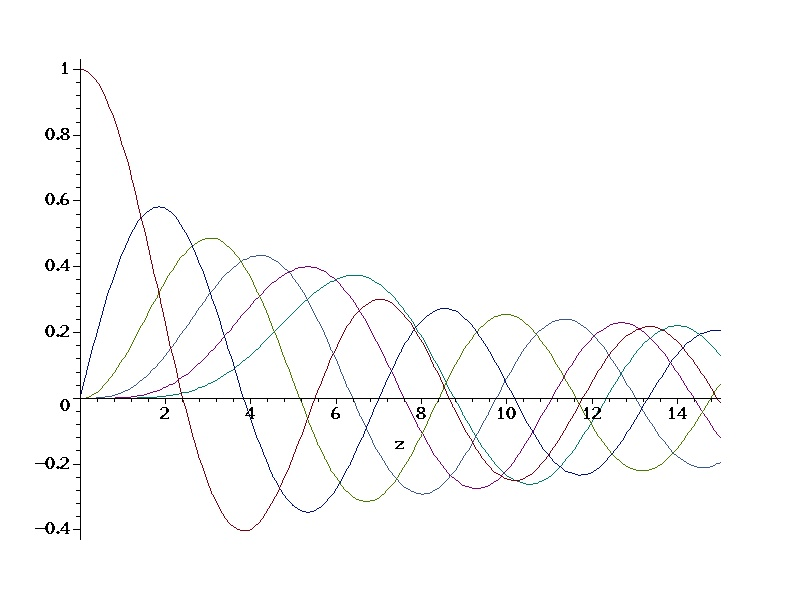
\includegraphics[width=6.4in]{example-04-fig.jpeg}}{Failed to create jpeg plot.}
   \captionof{figure}{The first six Bessel functions.}
\end{minipage}
\vfill

\clearpage

\pgfplotsset{compat=newest}
\pgfplotsset{width=0.45\textwidth,height=0.34\textwidth}

\subsection*{Using pgfplots}

\begin{minipage}[t]{\textwidth}
   \centering
   \begin{tikzpicture}
      \begin{axis}
         [xmin= 0.0,  xmax=15.0,
          ymin=-0.45, ymax=1.05,
          xlabel=$x$, ylabel=$J_n(x)$,
          grid=major, grid style={dashed,gray!30},
          legend entries = {$J_0$, $J_1$, $J_2$, $J_3$, $J_4$, $J_5$}]
          \addplot[blue]   table [x index=0, y index=1]{example-04.txt};
          \addplot[red]    table [x index=0, y index=2]{example-04.txt};
          \addplot[green]  table [x index=0, y index=3]{example-04.txt};
          \addplot[teal]   table [x index=0, y index=4]{example-04.txt};
          \addplot[orange] table [x index=0, y index=5]{example-04.txt};
          \addplot[purple] table [x index=0, y index=6]{example-04.txt};
      \end{axis}
   \end{tikzpicture}
   \captionof{figure}{The first six Bessel functions.}
\end{minipage}

\vfill

\begin{latex}
   \begin{tikzpicture} % requires \usepackage{pgfplots}
      \begin{axis}
         [xmin= 0.0,  xmax=15.0,
          ymin=-0.45, ymax=1.05,
          xlabel=$x$, ylabel=$J_n(x)$,
          grid=major, grid style={dashed,gray!30},
          legend entries = {$J_0$, $J_1$, $J_2$, $J_3$, $J_4$, $J_5$}]
          \addplot[blue]   table [x index=0, y index=1]{example-04.txt};
          \addplot[red]    table [x index=0, y index=2]{example-04.txt};
          \addplot[green]  table [x index=0, y index=3]{example-04.txt};
          \addplot[teal]   table [x index=0, y index=4]{example-04.txt};
          \addplot[orange] table [x index=0, y index=5]{example-04.txt};
          \addplot[purple] table [x index=0, y index=6]{example-04.txt};
      \end{axis}
   \end{tikzpicture}
   \captionof{figure}{The first six Bessel functions.} % requires \usepackage{caption}
\end{latex}

\end{document}
